\documentclass[oneside]{book}

% Order packages in each section in alphabetic order
% Added some generally useful packages 
% At the end of the project, remove not needed ones

% General packages
\usepackage[english]{babel}
\usepackage{hyperref}
\usepackage[utf8]{inputenc}

% Layout and formatting packages
\usepackage[ruled,vlined]{algorithm2e}
\usepackage[toc, page]{appendix}
\usepackage[font=small,labelfont=bf]{caption}
\usepackage{fancyhdr}
\usepackage{float}
\usepackage[T1]{fontenc}
\usepackage[a4paper, total={6in, 8in}]{geometry}
\usepackage{listings}
\usepackage{makecell}
\usepackage{multicol}
\usepackage{soul}
\usepackage{textcomp}
\usepackage{wrapfig}
\usepackage{xcolor}
\usepackage{graphicx}

% Math packages
\usepackage{amsfonts}
\usepackage{amsmath}
\usepackage{dsfont}
\usepackage{mathtools}

% Some general page settings from 
% https://github.com/giacThePhantom/MolecularPhysics
\pagestyle{fancy}
\fancyhf{}
\lhead{\rightmark}
\cfoot{\leftmark}
\rfoot{\thepage}

\setcounter{secnumdepth}{5}

\lstset{
    frame=tb, % draw a frame at the top and bottom of the code block
    tabsize=4, % tab space width
    showstringspaces=false, % don't mark spaces in strings
    numbers=none, % display line numbers on the left
    commentstyle=\color{green}, % comment color
    keywordstyle=\color{red}, % keyword color
    stringstyle=\color{blue}, % string color
    breaklines=true,
    postbreak=\mbox{\textcolor{green}{$\hookrightarrow$}\space}
}
  % Place all packages in the prefix file

% Set up document info
\title{\Huge\textbf{Tissue Engineering \\ - Motta -}}
\author{
  Stefano Cretti\\
  \small telegram: \href{https://t.me/StefanoCretti}{@StefanoCretti} \\[3pt]
\small Github: \href{https://github.com/StefanoCretti/TissueEngineering.git}{https://github.com/StefanoCretti/TissueEngineering.git}}

% File structure to expand
% Files should be named #section #chapter chapterName
\begin{document}
\maketitle
\tableofcontents
  
    \chapter{General course information}
  \section{Textbooks}
    \begin{itemize}
      \item Scaffold for Tissue Engineering: Biological Design, Materials, and Fabrication
      \item Introduction to Tissue material interactions (PDF)
      \item Selected chapters from : Principles of Regenerative Medicine (prof. Atala) (PDF)
      \item Selected chapters from: Adult wound healing (Yannis), and Extreme Tissue Engineering
      \item Selected scientific papers
    \end{itemize}

  \section{Assessment}
    \begin{itemize}
      \item \textit{TODO Still trying to define exactly}
    \end{itemize}

  \section{Topics}
    \begin{itemize}
      \item Concept of therapeutic device, transplant or implant?
      \item From tissue substitution to tissue regeneration: Introduction to tissue engineering
      \item Biocompatibility: concept evolution, mechanism, new approaches
      \item Structure, function, of ECM, role in cell activity, Cell/ECM interactions
      \item Wound healing: repair, regeneration, scar tissue formation
      \item Foreign body reaction: immuno, inflammatory, blood coagulation, complement system ECM as a model for scaffold design: engineering biomimetic scaffolds
      \item Polymers, biopolymers, hydrogels, fabrication methods
      \item Material/biological system interactions
      \item Strategies to control scaffold vascularization
      \item Strategies in TE: from top down to bottom up approach
      \item Organ printing and cell encapsulation
      \item TE applied to 3D in vitro models and lab-on-chip: drug screen, cancer studies, personalized medicine.
      \item In vitro-in vivo evaluations: bioreactors
      \item Lectures in lab: practical demonstration on scaffold fabrication
    \end{itemize}
    \chapter{Basics of tissue engineering}

\section{Definition of tissue engineering}

  \subsection{First definition}
  At first, \textbf{tissue engineering} was defined as \textit{"A combination of principles and methods of life sciences with that of engineering, to develop materials and methods to repair damaged or diseased tissues, and to create entire tissue/organs replacements"} (1980s).
  This definition was soon outdated since it did not consider a fundamental difference:

  \begin{multicols}{2}
    \begin{itemize}
      \item \textbf{Repair} is the act of closing the wound, restoring the macroscopic structure; the tissue  formed during repair is often different from the starting tissue (scar tissue for instance), and thus the different properties undermine the function of the repaired area due to the different properties.
      \item \textbf{Regeneration} is also a way of closing a wound, but the structure is restored using cells of the same type as the starting one, therefore maintaining the functionality of the area.
    \end{itemize}
  \end{multicols}

  Tissue engineering in fact aims at regenerating the structure and functionality of the district, not merely closing the wound.

  \subsection{Regeneration-centric definition}
  A following definition puts the focus on the regeneration aspect, underlining the necessity to understand the mechanism guiding regeneration: \textit{"The applications of principles and methods of engineering and life sciences, to obtain a fundamental understanding of structural and functional relationships in novel and pathological mammalian tissues, and the development of biological substitutes to restore, maintain or improve tissue function"}(late 1980s).

  \subsection{Current definition}
  Nowadays, tissue engineering could be defined as \textit{"a biomedical engineering discipline that uses a combination of cells, engineering, materials, methods and suitable biochemical and physicochemical factors to restore, maintain, improve or replace different types of biological tissues."}
  Tissue engineering holds promise of producing healthy organs for transplant by using patient cells (or immuno compatible cells). Tissue engineering can be combined with gene therapy, therefore including the correction of incurable genetic defects (such as sickle cell anemia).


\section{History of tissue engineering}
Tissue engineering is born from the concept that interaction between cells and extracellular matrix is important for understanding the structural and functional relationship of these components.
The first experiment on tissue engineering was conducted by W.T. Green, who tried to regenerate bone using chondrocytes (since in the physiological process, bone is obtained by calcification of cartilage); he managed to obtain bone formation in nude mice, thus he concluded that with the advent of innovative biocompatible materials it would be possible to generate new tissue by seeding viable cells onto appropriately configured scaffolds.
Later on, Langer and Vacanti created artificial scaffolds for cell-delivery, rather than using natural derived scaffolds which are difficult to replicate. The use of artificial matrices specifically designed for the system allowed to obtain reproducibility and high-quality.
(\textit{Skipped other experiments and history of tissue engineering})

\section{The need for tissue engineering}
Tissue/organ transplant is a heavily limited solution for tissue/organ failure; some of the main limitations being:

\begin{multicols}{2}
  \begin{itemize}
    \item Donor-recipient compatibility: it is almost impossible to find a fully compatible donor (all major histocompatibility complexes matching with the recipient) and the use of non-fully compatible organs/tissues requires the recipient to undergo immunosuppresive therapy (generally chronically) to avoid rejection of the transplant.
    \item Rejection risk: rejection can occur regardless of compatibility and immunosuppressive therapy, therefore this risk can never be avoided completely.
    \item Organ/tissue scarcity: even not considering compatibility, the amount of organs/tissues that can be donated is very scarce, since most of them come from car accident victims or relatives.
  \end{itemize}
\end{multicols}

For this reasons implanting artificial devices has grown more popular since:

\begin{multicols}{2}
  \begin{itemize}
    \item They are ready to use.
    \item They immediately restore the function of the organ/tissue.
    \item They can be personalyzed.
    \item They do not cause rejection.
  \end{itemize}
\end{multicols}

Still, implants present many limitation:

\begin{multicols}{2}
  \begin{itemize}
    \item They require invasive surgery.
    \item They can cause foreign body reaction.
    \item They cannot replace completely the functions of the organ/tissue (limited performance).
    \item They have limited duration.
  \end{itemize}
\end{multicols}

  \subsection{Examples of implant devices}
  Some examples of implant devices are:

  \begin{multicols}{2}
    \begin{itemize}
      \item \textbf{Hip joint prosthesis}: made of metallic alloys (mostly based on titanium) and ceramic (for the joint socket).
        It immediately restores the function of the joint but it requires very invasive procedures (long segment inside the femur) and overtime it sticks to the bone, making it really hard to substitute it.
        This last point is of little relevance if we consider older people, but it is a big problem for younger ones.
      \item \textbf{Vascular stent}: a stent is a cylindrical tool that is used in angioplastic procedures, meaning it prevents the stenosis (blockage) of (usually coronary) arteries.
        A flexible probe mounted with a stent, a balloon and some way to visualize the probe from outside the body (via ecography for example) is inserted in the femural artery; then the probe is navigated to the damaged region and the balloon inflates positioning the stent.
        This allows to restore blood flow to the miocardium without open heart surgery, even in an emergency setting such as in case of heart attack.
        The main problem is that the artery keeps contracting and expanding, therefore the stent can damage the vessel causing necrosis, proliferation of fibrotic tissue, inflammation; one way to reduce the problem is to use polymers rather than metallic alloys, since they are more flexible, but they are also less durable.
        Moreover stents are in contact with the blood and thus provide an abnormal surface that can start platelette aggregation and coagulation, creating blood clots; the use of slow release anticoagulant drugs stents helps with that aspect.
      \item \textbf{Artificial heart}: heart shaped device with valves.
        This device does not work as a pump since it cannot contract like miocardial fibres, therefore it require some form of auxiliary external pump.
        Just like with stents you can have abnormal coagulation on the surface of the device or due to turbolences in the blood flow.
      \item \textbf{Bone scaffolds}: they are three-dimensional biomaterial structures used for bone defect reconstruction.
        An ideal scaffold should have features such as improving cell adhesion, proliferation, osteogenic differentiation, vascularization, host integration and, where necessary, load bearing (drugs for instance).
        These design parameters should lead to specific scaffold properties, which include biocompatibility, porosity, micro and nano-scale structure, degradation rate, mechanical strength, and growth factor delivery, all of which dictate the biomaterial to be used or developed (\textit{further explaination later on}).
    \end{itemize}
  \end{multicols}

\section{Tissue engineering paradigma}
Since artificial devices do not replace all the functions of a lost organ or tissue and often fail in the long term, a new approach stems from two considerations:

\begin{multicols}{2}
  \begin{itemize}
    \item Living tissues and organs can be routinely assembled and reliably integrated to the body to restore, replace or enhance tissue and organ functions.
    \item Biomaterials can interact with living tissue and influence cell function and response.
  \end{itemize}
\end{multicols}

This approach is in fact tissue engineering which is, using yet another definition for it, \textit{"creation of a new tissue for therapeutic reconstruction of the human body, by the deliberate and controlled stimulation of selected target cells, through a systematic combination of molecular and mechanical signals"}.
Basically you are not creating ex novo a tissue/organ to implant, but you are inducing some biological mechanisms that helps the body heal itself; this idea is more generally represented by the term \textbf{regenerative medicine}, which includes not only tissue engineering but also cell therapy and gene therapy.
The main actors involved in this process are:

\begin{multicols}{2}
  \begin{itemize}
    \item \textbf{Cells}: generally stem cells derived from the patient (to avoid rejection).
    \item \textbf{Scaffold}: which is the structure used to induce and guide the growth of the cells; tissue engineering focusses mostly on material, surface and properties of this component.
    \item \textbf{Time}: required in order to induce and obtain regeneration in unnatural conditions.
  \end{itemize}
\end{multicols}

  \subsection{Scaffold characteristics}
  The main characteristics of a scaffold that must be considered are:

  \begin{multicols}{2}
    \begin{itemize}
      \item \textbf{Mechanical properties}: ability to withstand mechanical stress (elasticity, compressibility...).
      \item \textbf{Morphology}: shape, size, structure...
      \item \textbf{Physical properties}: behaviour when temperature, pH and other aspects of the environment change.
      \item \textbf{Histology}: type of tissue it has to replace.
      \item \textbf{Porosity}: permeability of the structure to different elements; it must allow the cells of interest to grow and penetrate into the structure while keeping outside unwanted cell types.
      \item \textbf{Water content}: the structure must contain enough water to allow nutrients to reach all the cells.
      \item \textbf{Surface}: the surface of the scaffold must be functionalized with molecules that are recognized by surface receptors of the target cells, thus inducing gene activation and some form of response (adhesion, expression upregulation/downregulation...).
    \end{itemize}
  \end{multicols}

  From these premises we get the so called \textbf{tissue engineering paradigma}, which is the basic flowchart that most tissue engineering procedures follow.
  In general, the main steps are:

  \begin{multicols}{2}
    \begin{itemize}
      \item \textbf{Collecting and isolating host cells of interest}: the type of cells needed for the procedure depends on the damage site; according to the cells needed (generally stem cells, sometimes primary cells) a biopsy is performed on an adequate tissue (blood, skin...).
        Moreover, since tissue are generally heterogeneous, some steps are required to isolate the cells of interest from the others.
        The fact that donor and recipient coincide, there are no compatibility issues.
      \item \textbf{Seeding cells on a scaffold}: the cells are then seeded on a scaffold made of some biomaterial which is biocompatible for the application at hand (\textit{biocompatibility characteristics are discussed later on}).
        This scaffold must provide adequate conditions for cell growth and proliferation, such as the presence of growth factors and cytokines.
      \item \textbf{Cell stimulation in a bioreactor}: The seeded scaffold is then placed into a static or dinamic bioreactor which induces and stimulate cell growth and proliferation.
        This bioreactor must be able to provide all the stimuli needed for cell differentiation and organization according to the desired final result (this may include mechanical stress for instance, needed for miocardial differentiation, or type of surface, since the differentiation of chondrocytes depends on the form they assume due to adhesion).
      \item \textbf{Re-implantation}: the fully prepared and populated construct is then implanted into the damaged area, where it will integrate itself with the surrounding tissues.
    \end{itemize}
  \end{multicols}

  This approach has some major downsides, namely:

  \begin{multicols}{2}
    \begin{itemize}
      \item It is very \textbf{labour intensive} and \textbf{time consuming} since it takes time for the cells to proliferate and populate the scaffold, moreover the growth conditions depend on the cell type of interest (which can be difficult to define, since the whole physiological environment must be taken into account, therefore angiogenesis, immune system, vacularization, lymphatic system and much more).
      \item Given the production time, this approach is \textbf{not ready to use}, therefore it cannot be used in an emergency setting.
      \item The amount of time and labour needed for the production implies \textbf{high cost}.
    \end{itemize}
  \end{multicols}

  In some cases, it is possible to simplify the procedure by implanting the scaffold immediately after it was populated with cells in the damaged area; this is called \textbf{in-situ regeneration}.
  In situ regeneration requires way less preparation time (almost ready to use) and uses the body of the recipient as a bioreactor, therefore reducing labour (you already have all the machinery required), need for bioreactor setup and overall costs.
  Notice that model animals cannot be used as bioreactors, since the mechanical properties of the tissues are not comparable (vertebrae of pigs and sheeps are built to support different weights compared to the human ones), the use of primates is strictly regulated by law and no animal is perfectly compatible with humans (therefore you risk rejection).
  The in-situ regeneration approach is not always applicable and just like the slower version it has a lot of room for improvement, for instance the development of more functional and durable polymers to use as scaffolds.
  Another problem for both strategies is the need of starting material, generally stem cells: the patient may not have enough excess tissue for an autologous transplant for instance.
  One way to mitigate this problem would be to save part of the umbilical cord to extract staminal cells, but in Italy this is forbidden by law (\textit{as of writing the notes}).

\section{Tissue engineering approaches}
There are two different \textbf{approaches} for tissue engineering:

\begin{multicols}{2}
  \begin{itemize}
    \item \textbf{Top-down approach} (traditional approach): cells are harvested from the donor, cultured and modified if needed. They are then seeded on a porous scaffold that during cell proliferation is slowly degraded by the cells and replaced by extra cellular matrix (ECM). The engineered tissue is then implanted into the patient. The main advantage of this procedure is that it is possible to produce mechanical stress, which is needed for the differentiation on certain types of cells.
    \item \textbf{Bottom-up approach} (modular approach): Some fundamental elements, such as cell sheets, cell aggregates, cell laden modules and bioink (3D printer ink containing cells) are used to construct a 3D module assembly, which can then be implanted into the patient. This modular building process allows to create very complex structures, with gradients and without a scaffold. Since a temporary gelatinous matrix is used, the module assembly lacks the rigidity provided by a scaffold, therefore it does not easily maintain the mechanical stress. Furthermore, when 3D printing, many other aspects have to be taken into account, like the permeability of the matrix to nutrients, the sensibility of the cells to the stress due to the extrusion from the needle and others.
  \end{itemize}
\end{multicols}

    \chapter{Biocompatibility}

\section{Introduction}
Biocompatibility is an essential aspect to take into consideration for the specification of the medical device that is being designed.
Before building a scaffold or a biological device its time, location and individual in which it will be used need to be defined.
A scaffold to be useful should activate specific cellular function and reflect and exploit the different mechanical and chemical properties of the tissue in which it will be implanted.
Because of this a scaffold it's designed taking into account the specific region in which it will be implanted considering the cell population and kind of injury among other parameters.
Cells are the building blocks of biology and they can read the information coming from the external environment.
Specific gene expression is activated in cells given external signalling molecules.
This makes it evident that the environment reaches the cell through chemical and mechanical stimuli.
Because of this scaffold are not self-sufficient entities: they are bioactive and need to collaborate with environment, cells and the extracellular matrix to perform their function.

	\subsection{Parameters defining biological outcome}
	The biological outcome that will be obtained then depends on a list of parameters which, once defined allow for the creation of a scaffold capable of regenerating the injured tissue.
	This parameters are:

	\begin{multicols}{2}
		\begin{description}
		\item[Porosity] is extremely important for cell migration.
			The material should be 3D for the cells, meaning that the scaffold should allow and promote cell adhesion, growth and migration.
		\item[Mechanical properties] are different for each tissue, the scaffold should both resist physical stress and provide the correct stimulus that the cells need to grow, adhere, migrate and differentiate.
		\item[Surface] modification is often referred to the functionalization of the scaffold through the addition of proteins or sequence of aminoacids to increase adherence.
		\item[Antibiotic/antiviral] drugs release system, to control chronic inflammation and possible infections.
		\item[Surface topography] may be smooth or rough for example.
		\end{description}
	\end{multicols}

\section{Guided tissue regeneration}
In the figure we can see articular cartilage, an intermidiate zone and bone. These three different tissues present differences in vasculartion, cell organization (in cartilage cells live in lacuna, where migration and proliferation are downregulated) and innervation.
\\
If the damage reaches the bone (which happens most of the times, because the cartilge does not have innervation, while bone does), the scaffold needs to account for different types of tissue. A multicomponent scaffold is designed, something that upregulates angiogenesis in the bone and downregulates it in the cartilage, that has high resistance to mechanical stimulations (cartilage has more water, material reaching water with hydrofilic properties). It should also provide for an enviroment for osteoblasts, lacunae for cartilage cells, space for nerves, vascularity and migration. It also needs to have different degradation times.
\\
The next step is check the biocompatibility, which will have an impact on cell adhesion, proliferation, differentiation, and also migration; on neoangiogenesis (spefic function) etc. Difference between regeration and repair (no/presence of scar tissue).

\section{The principles of tissue engineering}
%immagine triangolo
A tissue engineering process is composed by three steps:

\begin{multicols}{3}
	\begin{itemize}
		\item Design.
		\item Material choice.
		\item In vitro and in vivo testing.
	\end{itemize}
\end{multicols}

Tissue engineering implements a multidisciplinary strategy and the advance in materials' science and biology drastically improve the success of scaffold application.
Just consider how much the progressive knowledge in biology incremented the one in biocompatibility.
For example, M1 and M2 macrophages were only discovered in 2000.
But also the invention of polymers that can change their activity based on the environment (thermo/ph responsive), instructional (functionalization, e.g. with peptides that can control the cells' fate) and that can have specific mechanical strength and function (mechanical signalling).
In particular, the materials that can satisfy those requirements are considered 4th generation "biological regenerative biomaterials".
\\
Biomaterial need to be stable and inert in the beginning to be able to deliver drugs, to be used to print organ and used for cell therapies.
The hope for the future is to develop also diagnostic systems and to implant electronic devices, but one thing must always be present: biocompatibility.

	\subsection{Biocompatibility: a definition}
	At first, a material is biocompatible when inert, a ghost in the body: "the total absence of interaction between the material and the tissues".
	The minimal reaction to the foreign body was preferred, meaning no (or low) inflammatory reaction, no immuno-response.
	Definition focused on the body reaction to the implant and what was required was simply the chemical stability by the time.
	\\
	%immagine valvolve incrostate
	People however changed idea based on what they discovered after seeing what happened in the body after some time after implantation.
	Heart valve made of titanium and polyester failed because around the plastic layer the body built a very thick scar tissue and the valve could not open any more.
	The same valve in another patient induced trombosis.
	This first valve was treated with anticouagulants.
	The context of implantation is extremely important.
	A biological heart valve was harvested from pigs, but it failed because of calcification which rendered the valve unable to close.
	All the material induce a biological reaction.
	No material is completely inert, because our antibodies can recognize anything that is not "self".
	\\
	The concept of biocompatibility was revised: the ability of a material to perform a specific application causing an appropriate host response in a specific application” (1987).
	\\
	%immagine FBRx
	We can take as an example FBRx (cos'è?????), a non porous scaffold material.
	Depending on the chemistry of the material a specific protein adsorption is activated and subsequently an immune response.
	But if the material is not degradable, the macrophages start to coat the foreign body with scar tissue.
	At this point the reaction is finished.
	If the scaffold degrades eventually we will have an empty bag.
	Just by changing the porosity the scar tissue is reduced and regeneration is promoted.
	\\
	Injectable gels (hydrogel) are useful when filling cavities, becomes scaffold and supply for a scaffold for cells to migrate to.
	\\
	Take home lesson: scaffold should be tissue-organ dependent, defined situation, specifically react with the tissue (induce activation of cellular function to heal in a specific environment), material degradation.

	\subsection{Re-evaluation of the biocompatibility concept}
	Some factors led to the redefinition of the concept of biocompatibiliy, as for the scaffold is not enough to simply "exists":

	\begin{multicols}{2}
		\begin{itemize}
			\item Response to specific materials could vary from one application site to another (tissue-organ dependent) and not just on the material characteristics but it should also defined the situation in which the material is used (pathology, function).
			\item An increasing number of applications require that the material specifically react with the tissues rather than be ignored by them.
				Some applications required that the material degrade over time in the body rather than remain indefinitely.
			\item
		\end{itemize}
	\end{multicols}

	Most advance concept: biocompatibility is not a material's property but a system's property. It cannot be defined without considering the context.

\section{The complexity of the biocompatible system}
%immagine triangolo con tanta roba
Tissue engineering as a triangle: it seems easy with only three actors.
Each one has many possibilities!
\\
For a scaffold to be biocompatible the following steps must be followed:

\begin{multicols}{2}
	\begin{itemize}
		\item Determination of native tissue-organ.
		\item From in vitro to in vivo (from smaller to bigger animals, that depending on the biological problem).
		\item At this point we need to define the surgical model and finally we move to clinical trials.
		\item In addition, for in vitro test now bioreactors are used, because we don't want steady conditions but we want mechanical stimuli (the perfusion provides stress but also washes away cell residues).
	\end{itemize}
\end{multicols}

	\subsection{ECM molecules production: effect of the mechanical stimuli}
	%Immagine paper
	Different sponge-like scaffolds were produced with different properties (like porosity) for cartilage regeneration.
	The quality of GAG (mainly into the ECM of cartilage) was assessed.
	In addition, microCT to see where the GAG is and the sponges are completely infiltrated with it.
	SL500 had a lot of green (GAG) but only on the outside.
	What happens if the devices undergoes a mechanical stress similar to the biological situations? We get the exact contrary! Just by changing from a static to a perfusion situation.
	By changing the environment we ultimately change integrins and biological performances.
	In perfusion, the integrins were upregulated! Integrins are transmembrane proteins: portion inside and outside and are important so that scaffolds are able to talk to cells, instructive behaviour.
	Cells are extremely sensitive.
	In the very first case the in vitro model was not well designed.
	We must perform extensive and well thought tests before moving to the application.

    \graphicspath{{chapters/ecm/}}
\chapter{ECM}

\section{ECM functional role}
The functional role of the extracellular matrix in tissue engineering involves providing a starting point for scaffold biodesign.
The ECM is a dynamic environment, which is produced and regulated by cells.
The ECM performs the following functions:

\begin{multicols}{2}
	\begin{itemize}
		\item aids in cell locomotion: cells in the body are in movement, mediated by the action of receptors (transmembrane proteins) and ligands into the ECM. The ECM should provide ligands for adhesion, which should be patterned in order to direct the cells in a specific place;
		\item transmits and distributes mechanical loads: the ECM, depending on the tissue and mechanical stimuli, should assume a specific structure in order to transmit the stress to the cells, without damaging the cells. Considering the scaffold design, this means that the mechanical properties of the scaffold are really important. The best mechanical properties to reproduce depend on the context;
		\item prevents premature mechanical failure;
		\item partitions cells and tissues into functional units;
		\item acts as a scaffold defining tissue and organ architecture;
		\item acts as a storage and dissipative device for elastic energy;
		\item acts as substrate for cell adhesion, growth, and differentiation: cell adhesion is really important, and should be provided even for cell growth and differentiation, because cells are adhesive dependant - especially cells for regeneration. This means that activation requires adhesion.
	\end{itemize}
\end{multicols}

\noindent
The ECM is a controlled complex network. It is formed by a complex network of proteins, glycoproteins and proteoglycans, which together provide tissue specific biophysical and biochemical properties. Remember that the ECM is tissue specific. The contact between the nucleus and the ECM is performed by integrins. We must find which genes should be activated for stimulating regeneration and the ligands for gene activation.
\\
\noindent
The ECM must interact with the cells. If the interaction is interrupted, the cells may go into pathology.
The ECM provides not only mechanical and structural support to cells and tissues, but also binds soluble ligands and transmembrane receptors to provide spatial coordination of signalling processes.
The ability of cells to sense the chemical, mechanical and topographical features of the ECM enables them to integrate complex, multiparametric information into a coherent response to the surrounding microenvironment.
Consequently, dysregulation or mutation of ECM components results in a broad range of pathological conditions.
\\
\noindent
The ECM is a composite material where cells sense the environment.
An example is a chondrocyte in a bone-like environment that will transform into bone, via calcification.
We need to pay attention to not having a damage effect instead of a therapeutic effect.
ECM polymers/network are instructive,  they provide structural and mechanical integrity to tissues.

\section{Components of the ECM}
\begin{itemize}
\item Physical signals are from fibronectin, vitronectin, collagen, laminin, fibrillin, GAGs, PG,...
\item Soluble signals: CF, cytokines, chemokines,...
\item Structure: composites, fiber-based, function dependent
\item Water: used to better tune mechanical properties. It can help the material to support the stress. Water is highly present in articular cartilage! The molecules able to ligate the water are GAGs and PGs. More water means more GAGs and PGs.
\item Mechano-transduction: translating mechanical stimuli
\end{itemize}
\noindent
Fibers are made of collagen, which can form fibrils (very elastic structures), fiber (a little bit thicker) or bundle (composition of more fibers all together). In addition, to better tune the mechanical properties without changing the chemistry, nature can also change the organisation of the fibers: they can be well oriented or randomly distributed, depending on the mechanical stimuli and the direction of them.
\\
\\
\noindent
Signals are important for the adhesion, so other molecules are introduced into the scaffold as well, adhesion ligands and collagen (to form the structure, it is able to provide ligand too).
Another strategy is trying to reduce the number of the elements, in particular the number of the molecules produced by the cells. How? By designing multi-functional polymers, one polymer must do many things. Finally, it is possible to employ soluble signals. Cells can communicate with each other - very distant cells communicate thanks to soluble signals.
\\
\\
\noindent
Thanks to the cross-talk between cells and ECM we have the trigger and the control of many processes. ECM/cells crosstalks facilitate and regulate: pattern formation, morphogenesis, cell fate, daily cellular processes, wound healing, tissue homeostasis.

\subsection{Stem cells}
The environment is important even for stem cells. Stem cells are rare cells that are uniquely capable of both reproducing themselves (self-renewing) and generating the differentiated cell types that are needed to carry out specialised functions in the body.
This is important in the embryogenesis and a balanced control between self-renewed cells and differentiation is fundamental in the healing process and homeostasis. If it is deregulated we can have tumorigenesis, degeneration, pathology,...
Pay attention: the scaffold sends information, we can induce cancer formation too!
Changing the organization of the fibers in the ECM leads to modifications in water content and rigidity ; as a result, we will end up with a completely different signal.

\section{The matrixome: chemistry of the ECM}
\begin{figure}[ht]
\centering
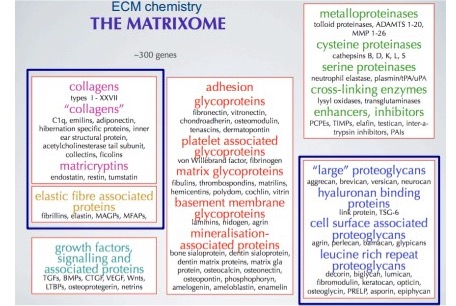
\includegraphics[width=0.8\textwidth]{matrixome}
\caption{\label{fig:matrixome}}
\end{figure}

\noindent
The stiffness is controlled by collagens, elasticity by elastic fibers.
Signalling molecules are used for cell-cell communications e.g. growth factors.
Adhesion molecules promote cell adhesion, pattern to drive the mobility direction.
The proteinases are important to destroy the proteins we don’t want, they provide dynamicity. The GAGs and PGs are relevant for the water content of the ECM.
Something important for scaffold design is that we can use proteinase to degrade the scaffold once we need to degrade it, not before.
\\
\noindent
Matricellular proteins are extracellular modulators of cell function expressed at high level during development and in response to injury. They are modulators of cell matrix interactions and bind to many cell surface receptors, the ECM, GFs, cytokines and proteases. Their role is to induce de-adhesion in contrast to the adhesivity of most matrix proteins (migration).
\noindent
Functions:
\begin{itemize}
\item cell adhesion, migration, chemotaxis
\item matrix assembly and collagen fibrillogenesis
\item regulation proliferation/apoptosis
\item binding/activation GFs and cytokines
\item angiogenesis and tumour growth
\end{itemize}

%Example: support of a state of intermediate adhesion (disruption of focal adhesion and reorganisation of actin stress fibers):	TSP1 and 2, Tenascin-C, SPARC
%Cercare più info/appunti

\section{Collagen}
Collagen is one of the most important proteins for the ECM, as it provides structural properties. Collagen is produced by cells: the production starts in the cytoplasm,  while the final assembly is performed outside the cell.
Fibrils are formed first, then assembled into fibers and bundles.
\noindent
How can collagen build the network?
\begin{itemize}
\item connective tissue: less density, soft network, more water, fiber and fibrils
\item meniscus: parallel fibers, more density, packed fibers, because of different functions, bundle (more stress)
\item myocardium: mechanical stresses, it should support the growth in one direction
\end{itemize}
\noindent
Cells can migrate in this low porosity material through a specific enzymatic process,  which allows the space to be opened up.
Collagen is non-homogeneous, bottom-up, multi-functional, dynamic and has a hierarchical structure. The structure is function dependent.
We have three chains,  which can reach a helix formation (quaternary structure). If we increase the chemical bridges between the helices we control elasticity.
\\
\\
\noindent
The ECM is degraded by cell-secreted proteases (remodelling) and releasing of bioactive component.
Natural ECMs modulate tissue dynamics through their ability to locally bind, store and release soluble bioactive ECM effectors such as GFs.
Our scaffold should promote cell migration.
\\
\\
\noindent
Collagen is a family of proteins, we have at least 23 different types of collagens, depending on the tissue we have the prevalence of one type on another type. In the cartilage for example we have collagen type II. In tendons we have type III collagen, which is really similar to jellyfish collagen, currently commercialized.

%add table
These are the proteins family into the ECM.
There are no changes in the chemistry, but in the ratio of the presence of one and the other.
For the scaffold: little changes can have a huge impact on the cells.

\section{Fibronectin}
Fibronectin is a large matrix glycoprotein present in most body tissues fluids.
Functionally, it is the classic example of an adhesive glycoprotein, binding and interconnecting extracellular matrix components with each other and to the surface of the cells.
It is one of the most important molecules through which cells interact with the surrounding environment.
The binding of fibronectin to the cell surface’s integrin receptors plays a critical role in the cell migration (during the development and postnatally).
\\
\\
\noindent
Fibronectin is made of two identical chains connected by a disulphide bond, a dimer.
We can recognise different sections:
\begin{itemize}
\item one can interact with fibrin and heparin
\item one can interact with gelatine and collagen
\item one can interact with the cell receptor (arg-gly-asp ac. sequence)
\item one can interact with polysaccharide heparin
\item one can interact with fibrin
\end{itemize}
\noindent
These molecules must be able to interact and crosslink because in this way if we have a stimulus that acts in the collagen, for example, the other parts of the ECM can sense said stimulus. In addition, many regions of the ECM are able to interact with cells, controlling the structure and cellular activity.
\\
\\
\noindent
In ECM we have fibronectins, collagen, gel-forming polysaccharides, water, actin and the cell (figure \ref{fig:structure}).
The transmembrane can sense what is going on in the external side and transfer the information to the internal part and eventually to the nucleus to activate a specific gene expression.
The interactions are important and interesting, the scaffold needs to provide the ability to interact with the same exact mechanism and cells must work in an appropriate way.
We don’t want dysregulation of the mechanisms and the tissue, so we need the natural mechanism of interaction.

\begin{figure}[ht]
\centering
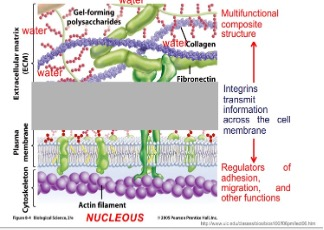
\includegraphics[width=0.6\textwidth]{structure}
\caption{\label{fig:structure}}
\end{figure}

\noindent
The ECM is a mosaic structure, a guide for cell functions.
Should the scaffold replicate the ECM? Partially, yes, but especially the functions! 
Large molecules are difficult to manage, maybe using a smaller molecule (nectin instead of fibronectin) is easier.
Fibronectin is needed to reproduce the complete ECM, but nectin is sufficient to promote cell growth.

\subsection{Fibronectin multifunctionality}
The RGD-loop is strategically placed to undergo strong conformational changes and constitutes a mechanosensitive switch for recognition by integrin receptors.
Depending on the mechanical stimulus, fibronectin can assume specific conformations, changing its activity.

\section{Proteoglycans and GAGs}

\textbf{Proteoglycan}: head core protein + chain of polysaccharides (GAGs), which is hydrophilic (figure \ref{fig:pgag}). 
Responsible for controlling the water content of the tissue.
They are especially important in case of mechanical stresses.
\\
\\
\noindent
\textbf{Glycosaminoglycans} (GAGs) are linked to the core proteins, we can have:
\begin{itemize}
\item hyaluronic acid
\item chondroitin sulfate
\item keratan sulfate
\end{itemize}

\begin{figure}[ht]
\centering
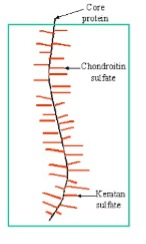
\includegraphics[width=0.3\textwidth]{pgag}
\caption{\label{fig:pgag}}
\end{figure}

\noindent
GAGs are made up of repeating disaccharides and have a large number of negative charges,.
They are already using some of these molecules in clinics, e.g. hyaluronic acid.
The big protein is able to interact with water.
The core protein, hydrophobic, is covered by hydrophilic molecules.
The water should be able to go out when the tissue undergoes mechanical stress to ensure homeostasis.
This is a reversible mechanism,  the scaffold must have specific properties to resist stress and control water flow.

\section{Modelling nature}
Our goal is to stimulate the cell.
The environment is dynamic, and the interactions are possible thanks to the water.
The interactions between cells and environment are relevant to regulate a lot of processes, from cell fate to tissue formation and regeneration.
Our scaffold will be one of the components that will collaborate to regenerate the tissue.
Once again, we need a model, which is nature.
We need to leave cells work in a natural way.
Living organisms naturally provide a multiplicity of materials, architectures, systems and functions, all resulting in from stringent selection process (evolution).
\noindent
Strategy:
\begin{itemize}
\item polymers (materials) able to integrate
\item molecular synthesis (by cells) at very high level of organisation (molecular recognition, multifunctionality, self-diagnostic, destruction-recycling, bottom-up approach)
\item structure (self-assembling, molecule interactions, interfaces, etc) dynamics
(responsive polymers, adaptation, self-healing)
\end{itemize}
\noindent
The bottom-up approach is more bio-mimetic,  as it reflects how nature works [self-assembling blocks, proteins are formed automatically from amino acids].
We should also focus our attention on building a context-specific microenvironment.
\\
\\
\noindent
Apoptosis is a programmed cell death, in which cells are encapsulated by vesicles and removed.
Necrosis instead happens when the cellular membrane is damaged, we have inflammation.
During necrosis the activity of macrophages is increased, producing also inflammation for neighbouring cells.
It has been suggested to induce tumour cell death through apoptosis to avoid upregulating inflammation.

    \graphicspath{{chapters/inflammation/}}
\chapter{Inflammation}

Biocompatibility is the ability of a material to perform with an appropriate host response in a specific application.
The first system interacting with the scaffold is the immune system, which first gives an immuno response and then starts the healing process. 
Such system can be different tissue by tissue, from healthy or pathologic tissue, etc.
A widespread idea derived from findings in diverse species is that the loss of regenerative capacity is linked to the evolution of immune competence. 
The relationship between tissue healing and the immune response is very complex, since there are both negative and positive roles, depending on the tissue, organ and life stage (embryonic, neonatal or adult). We need to try to reduce inflammation as soon as possible, in order to prioritize healing.
\\
\\
\noindent
If we have a wounded skin in a fetus we will have complete regeneration without scar tissue formation, whereas in adults we observe fibrotic healing. We can take some parameters from the fetal model to try to reduce as much as possible scar tissue formation in adult patients.

\section{Tissue damage}
During the inflammatory response (defence step) we have platelet activation, coagulation, inflammation, leading to bleeding, pathogens, open wound, cell debris. 
Our aim is to block the wound.
The body first triggers a coagulation cascade, then the system will be activated to regenerate. 
\\
\\
\noindent
In 3-7 days we have migration, proliferation, synthesis, angiogenesis. 
For pathogens we need scar tissue blocking the entrance; inside pathogens need to be addressed by internal inflammation, increase blood flow into the damaged site through angiogenesis (more capillaries).
The overall process is controlled by inflammatory system cells e.g. macrophages. 
Cells are coordinated by interleukines e.g. IL-1, IL-2.
\noindent
What kind of cells are involved? There are three major roles of complement:
\begin{itemize}
\item opsonize particles for phagocytosis (need only reach the C3b stage). Phages can recognize the mark through integrins.
\item elicit inflammatory reaction by acting on leukocytes, mast cells, endothelium
\item complement-mediated cytolysis
\end{itemize}
\noindent
The processes are described in figure \ref{fig:roles}.

\begin{figure}[ht]
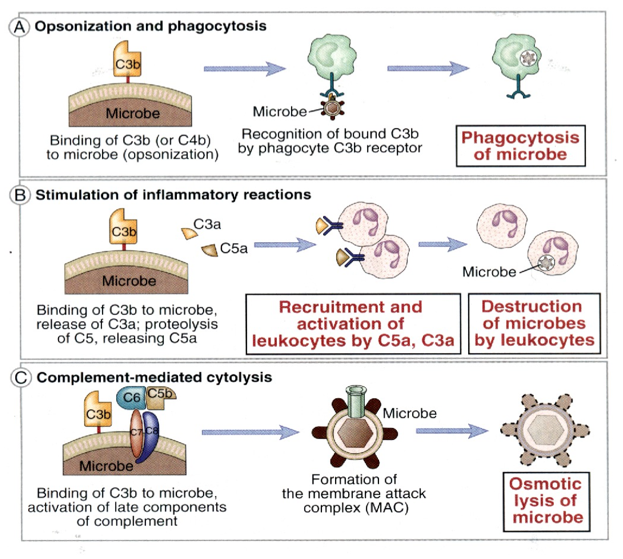
\includegraphics[width=0.6\textwidth]{roles}
\caption{\label{fig:roles}}
\end{figure}

\section{Leukocyte population}

\textbf{Neutrophils/polymorphonuclear} are the most abundant circulating leukocytes. 
There are 2 types of intracellular granules, which are common progenitors with monocytes. 
The adult human produces average of $10^{11}$ per day, with a short life span (6 hours and then apoptosis).
\\
\\
\noindent
\textbf{Monocytes} (and activated macrophages) are phylogenetically the oldest cells of the immune system. 
They circulate as inactive monocytes, enter tissue and become activated macrophages.
They are located in the subepithelial connective tissue, which is present in the interstitia of parenchymal organs, in the lining of vascular sinusoids in liver and spleen and in the lymphatic sinuses of lymph nodes.
Monocytes usually respond later than neutrophils at sites of injury/infection and are the primary effectors of innate immune system.
\\
\\
\noindent
The primary purpose of phagocytes is to clear invading organisms, foreign non-self materials. 
Monocytes can exist for years, while neutrophils live just a few hours.

\section{Phagocyte-mediated wound cleaning}
To produce new vessels from new cells, the mechanism of phagocyte-mediated wound cleaning is the following:
\begin{enumerate}
\item recruitment: adhesion proteins facilitate attachment to endothelium
\item migration: receptors that mediate chemotaxis to target site
\item recognition and phagocytosis: specific receptors for microbes and opsonized materials (phagocytosis) Fc receptors and C3 receptors are major mediators of attachment
\item release of cytotoxic compounds: reactive oxygen and nitrogen species
\item cytokine production secretion of numerous cytokines and chemokines with local and systemic activity:
	 \begin{itemize}
		\item positive factors: increase macrophage activation, recruitment, stimulate adaptive immune system
		\item negative factors: inhibit activation and proliferation
		\item secretion of factors that facilitate wound remodeling, matrix production and angiogenesis
	\end{itemize}
\end{enumerate}
\noindent	
Macrophages dominate biomaterial interfaces in tissue, often present chronically. 
They control the interaction of the scaffold with macrophages and avoid pro inflammatory signals.

\section{Leukocyte extravasation}
Leukocytes travel through blood capillaries. 
Signal molecules (chemotactic signals) first cause leukocytes to adhere to endothelial cells. 
An example of diffusible chemotactic signal are bacterial peptides resulting from bacterial degradation in the inflammation site.
The binding of integrins and I-CAM tightens the adhesion and triggers process formation (note this is an exception to the general role of Integrin-ECM interactions).
Additional signals/ligands promote migration.
The overall process is summarized in figure \ref{fig:leuko}.

\begin{figure}[ht]
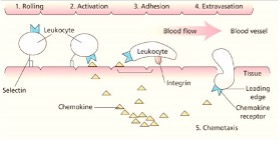
\includegraphics[width=0.7\textwidth]{leuko}
\caption{\label{fig:leuko}}
\end{figure}
 
\section{TNF alpha}
TNF is the principal mediator of acute inflammation.
Its major source are macrophages and its major effect is the activation of pro-inflammation NFkB transcription factor.
TNF increases the endothelial expression of selectins and integrins, the chemokine production in endothelial cells, macrophage and the production of prostaglandins and leukotrienes (pyrogens, chemotactic). 
Furthermore, it induces prostacyclin expression in endothelium, increases local blood flow and increase IL-1 production in macrophages.

\section{Inflammatory response}
The inflammatory response is the body’s natural response that occurs immediately following tissue damage.
 Its main functions are to defend the body against harmful substances, and to promote the renewal of normal tissue.
Signs of inflammation:
\begin{enumerate}
\item pain: due to chemical released by damaged cells
\item swelling or edema: due to an influx of fluid into the damaged region
\item redness: due to vasodilatation (widening of blood vessels and bleeding in joint or structure)
\item heat: due to an increase in blood flow to the area
\item loss of function: due to increased swelling and pain
\end{enumerate}
\noindent
The inflammatory reaction is the combination of a number of overlapping reactions within the body. 
Although a lot of these occur simultaneously, a certain order of events may be seen.
The tissue damage may occur from trauma such as a tackle, collision or from a fall. 
However, quite commonly tissue injury is as a result of overuse (microtrauma) or pathology
\\
\\
\noindent
When tissue cells become injured, they release a number of chemicals that initiate the inflammatory response. 
Examples of these are kinins, prostaglandin and histamine. 
These chemicals work collectively to cause increased vasodilation (widening of blood capillaries) and permeability of capillaries. 
This leads to increased blood flow to the injured site. 
These substances also act as chemical messengers that attract some of the body’s natural defence cells, in a mechanism that is known as \textbf{chemotaxis}.
Although highly beneficial to the body’s defence strategies, some chemicals also increase the sensitivity of the pain fibres in the area and so the area becomes painful.

\section{Leukocytes migration}
Chemotaxis leads to the migration of certain white blood cells to the damaged area. 
Two types of leukocytes are predominant in the inflammatory response (macrophages and neutrophils). 
Neutrophils are first to reach the injured site and function by neutralising harmful bacteria. Macrophages aid the healing process by engulfing bacteria and dead cells and ingesting them so that the area is clear for new cells to grow. 
They arrive at the injured site within the first 72 hours of the injury and may remain in the area for weeks after the injury.

\section{Wound healing in skin}
We have acute inflammation, proliferation, remodelling and then the reprise of the tensile strength. 
The synthesis of collagen occurs between 7 and 14 days. 
After 14-21 days, we have collagen cross-linking assembling. 
Less cross linking means more flexibility and less strength. 
There is a control of the immune system to induce tissue regeneration.
\\
\\
\noindent
At the beginning we have pro-inflammatory macrophages phagocyte (type I),  which produce cytokines. 
When all the debris has been removed, the macrophages type I become of type II, leading to the downregulation of pro-inflammatory cytokines and tissue regeneration.
Immune tissue engineering is a new approach to drive the transition from type I to type II in order to promote regeneration. 
We need to first release few pro-inflammatory molecules (short response) and then tune the transition.

\noindent
The main actors of the immune response following tissue injury:
\begin{itemize}
\item kinetic of immune cell mobilisation after tissue injury
\item initial inflammatory phase following tissue injury
\item immune mechanisms that can impair tissue healing or drive to scarring and fibrosis
\item pro regenerative immune mechanisms
\end{itemize}

\begin{figure}[ht]
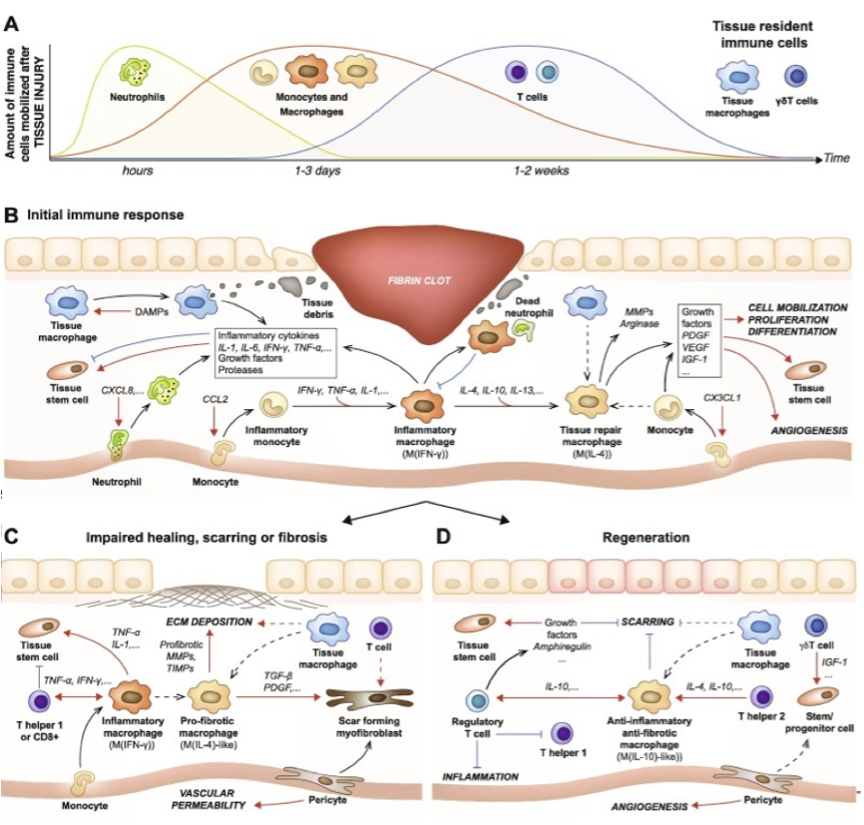
\includegraphics[width=1\textwidth]{healing}
\caption{\label{fig:healing}}
\end{figure}

\section{Strategies to promote tissue regeneration}
Strategies based on biomaterials and drug delivery systems to promote tissue regeneration by controlling the immune system:
\begin{itemize}
\item physicochemical properties of the scaffold. Pay attention to degradability, hydrophobicity, topography…
\item pro-inflammatory modulators
\item anti-inflammatory modulators
\end{itemize}
\noindent
Materials must be chosen according to	protein adsorption, generalised toxic effect, inflammatory cell activation, fibrosis, microvascular changes and tissue-organ specific cell response.

Specific application, tissue-organ type:
\begin{itemize}
\item activation of clotting cascade
\item platelets adhesion activation aggregation
\item complement activation
\item antibody production
\item immune cells response
\item hypersensitivity
\item mutagenesis, genotoxicity
\item tumor formation
\end{itemize}
\noindent
Everything is controlled by the material (type,shape, size, properties) and the environment.
When the biomaterial is recognized as a foreign body, macrophages are recruited and cells will not be able to migrate on the scaffold for regeneration, resulting in a complete failure.

\subsection{Effects of physicochemical modification to biomimetic scaffolds in musculoskeletal applications}
\begin{figure}[ht]
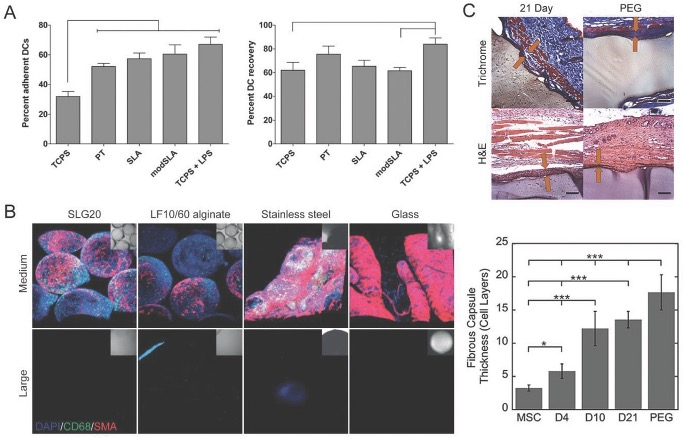
\includegraphics[width=0.9\textwidth]{muscosk}
\caption{\label{fig:muscosk}}
\end{figure}
In figure \ref{fig:muscosk} we can check the percentage of dendritic cells(inflammatory cells) in the sample. 
We can have a different adhesion degree of inflammatory cells to the scaffold. 
Buffering solution + serum (proteins) + antibiotics + growth factors…depending on the absorption we will have a different cell development. 
In panel B we see the different shape and thickness for each material.
%chiedere altri appunti su questo, poco chiaro

\subsection{Processes affect the biological outcome}
The aim of this experiment is to evaluate the ability an organic membrane to treat skin burn. Absorption is an important property to take into account, because it causes the inflammatory response. 
Keep in mind that proteins can assume different conformations according to specific situation. Three membranes were prepared, they look almost exactly the same. 
By increasing crystallinity, the water content is reduced,  leading to different mechanical properties (huge rigidity, increased hydrophobicity = less water absorption for the scaffold). 
In vitro tests of the material: fast, easy, not expensive. 
In this case they moved materials A and B into further clinical trials. When moving the material in vivo we will have the incubation with human plasma (reproduce bleeding); the aim is to focus on pro-inflammatory signals.
Chemical production: pro-inflammatory cytokines and mixed environment (pro and anti-inflammatory). Moving down there is increase in opsonin.  Some are stretched, as macrophages lead to more adhesion and activation. 
We observe low adhesion and high inflammation, this is induced by the material for the scaffold. A small amount of proteins is still able to induce a high pro-inflammatory reaction. 

\section{Major activities of macrophages secreted factors}
The main goal of the inflammatory response is healing. 
The system will pass through scar tissue formation, modification and finally regeneration. Macrophages react to inflammation through the killing of microbes (nitric oxide)and phagocytosis. 
%They should find oxotin, produced by the system.  ???
At the beginning we must defense our body from pathogens and next to build up.

\section{Inflammatory monocytes}
\begin{figure}[ht]
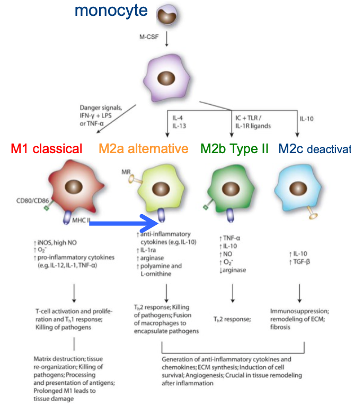
\includegraphics[width=0.7\textwidth]{mono_diff}
\caption{\label{fig:mono}}
\end{figure}
In figure \ref{fig:mono} we see macrophages differentiation from classical proinflammatory to regenerative. 
Each one is characterized by a specific chemistry. 
Maybe we can employ some of these molecules to witness which kind of macrophage is present. After the interaction between material and inflammatory cell, we must find which will be the inflammatory molecules produced afterwards. 
Sometimes scaffolds are able to produce new ECM, but not new capillaries. 
Our aim is to study when angiogenic factors should be released to induce the regeneration process. 
 
\section{Inflammatory cellular responses}
Opsonin provides the ability for a specific cell to hit the particles and digest them. Phagocytosis involves moving the foreign body from outside to inside within a membrane.
Cancer cells are recognised as foreign since they are coated by opsonin, so they will be eaten by phagocytes.  
Cellular responses: oxidative burst, bacterial killing, tissue injury. 
If the material is very sensitive, it will release pieces, which are destroyed by macrophages and necrotic surrounding tissue. 
The small particles will upregulate the inflammatory response, leading to chronic response. 
Our aim is to reduce as much as possible the intensity and time of the defence, the scar tissue.

\begin{figure}[ht]
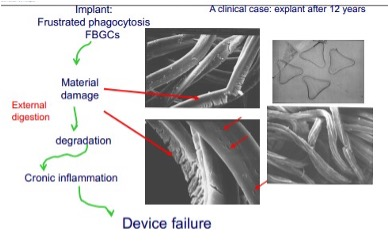
\includegraphics[width=0.8\textwidth]{failure}
\caption{\label{fig:failure}}
\end{figure}
\noindent
Figure \ref{fig:failure}: interaction between cells and material in an implant, explanted after 12 years due to failure.  
The tube changed its shape and diameter, provoking blood turbulence, thrombosis risk. 
The issue is that spaces were occupied by macrophages, which were able to adhere and digest the external fibers - released in microparticles. 
The prosthesis was made in nylon, which is considered to be the most stable polymer e.g. used for parachutes. 
Since it is stable and strong, the human body sensed it as foreign and started damaging it. T
he section of the damaged fibers was triangular, while circular fibers had no impact whatsoever. 
What does it mean to try to digest a foreign body? The phagocytes digest it piece by piece and this leads to chronic inflammation and failure.

\section{Tissue Healing}
\begin{enumerate}
\item collagenation and cartilarisation
\item angiogenesis
\item proliferation
\item remodelling
\end{enumerate}
\noindent
Once sufficient cleansing of the area has been achieved, the damaged area begins to sprout new capillaries to bring blood to the region - this is known as angiogenesis or revascularization. 
When blood flow has been re-introduced to the area, specific tissue cells begin to re-grow.
For example, in a muscle tear muscle cells will repopulate the area. 
Wound healing occurs towards the end of the inflammatory process, however the two processes overlap considerably. 
\\
\\
\noindent
Macrophages work to clear the damaged area and make space for the regeneration of the new tissue. 
After a number of days, fibroblasts (collagen producing cells) begin to construct a new collagen matrix which will act as the framework for new tissue cells.
Tissue healing occurs with the sprout of new capillaries to bring blood to the region (revascularization). 
Cellular responses in tissue repair: the capillary should not go randomly, the scaffold architecture should also consider space for angiogenesis.
 We must also ensure a path for interconnection by playing with architecture and release of angiogenetic factors.
\\
\\
\noindent
The proliferation phase lasts 4 weeks.
In cases where the injury has been more severe, the affected area may be composed by a mixture between specific tissue cells (such as muscle cells) and other tissue known as granulation tissue. 
If this granulation tissue is not removed it will remain and form scar tissue, which can lead to a decreased functional ability of the tissue.
\\
\\
\noindent
The remodelling occurs when the new cells mould into their surrounding to once again produce a functional tissue. 
This process of remodelling can take months even years, altering the new tissue slowly. 
The new cells and protein fibers become arranged in a way that is best suited to the stresses imposed on the tissue. 
Hence, when a tissue is healing ,it is important to stretch it in the correct direction so to optimise the strength of the new tissue.

\section{Rethinking regeneration: empowerment of stem cell by inflammation}
Immune cells at the site of tissue injury, including macrophages and T cells, secrete TNFalpha, TNFy, IL-1, IL-13 and other pro-inflammatory cytokines, which in turn can activate stem cells. 
Once licensed by these cytokines, stem cells can facilitate tissue regeneration though cell differentiation and the release of anti-inflammatory cytokines and growth factors.

\section{Designing immuno informed biomaterials matrices}
We need to provide safety paying attention to tumorigenesis.
There is also the use of extracellular vesicles to load drugs.
We can play with the surface topography or chemistry to design the matrix.
Another aspect that we need to take into account is the macrophage polarization and network formation.
The network should be formed in 3D on the surface, interconnections for macrophages.
For instance, if we have an implanted scaffold we first observe protein adsorption. 
After this we have adhesion, macrophages can adhere by forming a network speeding up the process towards regeneration. 
Macrophages are also involved in vascularization. 
When the scaffold is not porous the macrophages will not be able to polarize and switch to state II, they induce the formation of scar tissue.

\section{Effect of topography and stiffness on macrophages polarisation}
Macrophages assume an elongated shape, M2 like phenotype (up-regulated expression of arginase), on PDMS substrates with 2 gratings topography compared to planar control.
After the adhesion (f), cells start to polarize (g) [figure \ref{fig:topo}] .  Increased stiffness in hydrogel drives the transition in absence of cytokines stimulation. 

\begin{figure}[ht]
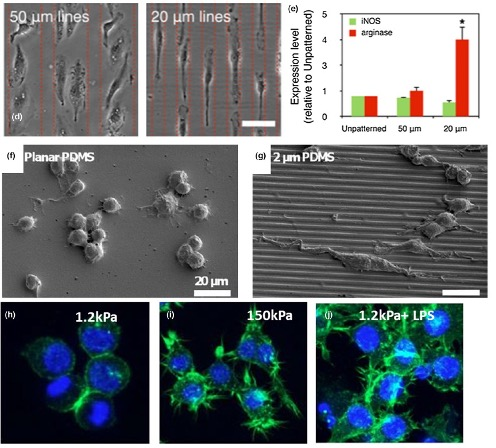
\includegraphics[width=0.8\textwidth]{topo}
\caption{\label{fig:topo}}
\end{figure}

\section{Role of pore size/distribution/degradation}
\begin{figure}[ht]
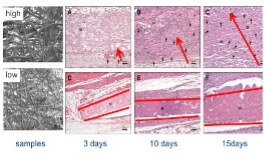
\includegraphics[width=0.8\textwidth]{silk}
\caption{\label{fig:silk}}
\end{figure}

Figure \ref{fig:silk}: silk fibroin micro-nets formic acid treated (in vivo evaluations). 
In this case we have induced regeneration in unnatural conditions. 
Changing the pore size, the mechanical properties will be affected. In high porosity samples: after 3 days we have granulated tissue (dots are cells), the scaffold was able to promote movement inside. 
At 10 days the arrows are indicating new capillaries. 
Macrophages are at phase II, cells have more space to build tissue. 
Then thinner fibers, blood vessels, not so many dots, signalling that inflammatory cells almost disappeared. 
Already after 3 days we have a very clear scar tissue formation, which becomes thinner in 10 days. 

We have also different vascularisation and degradation that depend on porosity.

    \graphicspath{{chapters/biorecognition/}}
\chapter{Biorecognition}

\section{Molecular Biorecognition}
Tissue engineering and regenerative medicine require an intimate understanding of the native ECM, together with the complexity of cell and tissue biology. For therapeutic applications, we should mimic the basic structure of ECM using a variety of synthetic or naturally derived materials and fabrication methods.
The scaffold can be seen as a 3D growth environment:
\begin{itemize}
\item basic structural properties of ECM
\item molecular cues to control bio responses
\item protease sensitive site for enabling migration
\item locally delivery of soluble factors for tissue remodelling stimulation
\end{itemize}

\subsection{Functions of the ECM}
\begin{itemize}
\item aids in locomotion
\item transmits and distributes mechanical loads
\item prevents premature mechanical failure
\item partitions cells and tissues into functional units (scaffold architecture)
\item acts as a scaffold that define tissue and organ architecture
\item acts as a storage and dissipative devices for elastic energy
\item acts as substrates for cell adhesion, growth and differentiation
\end{itemize}
These functions are defined by composition, structure, mechanical properties and repair response, which depend on tissue type, physiopathology, mechanical forces, damage and healing process. 
\\
\\
\noindent
\begin{figure}[h]
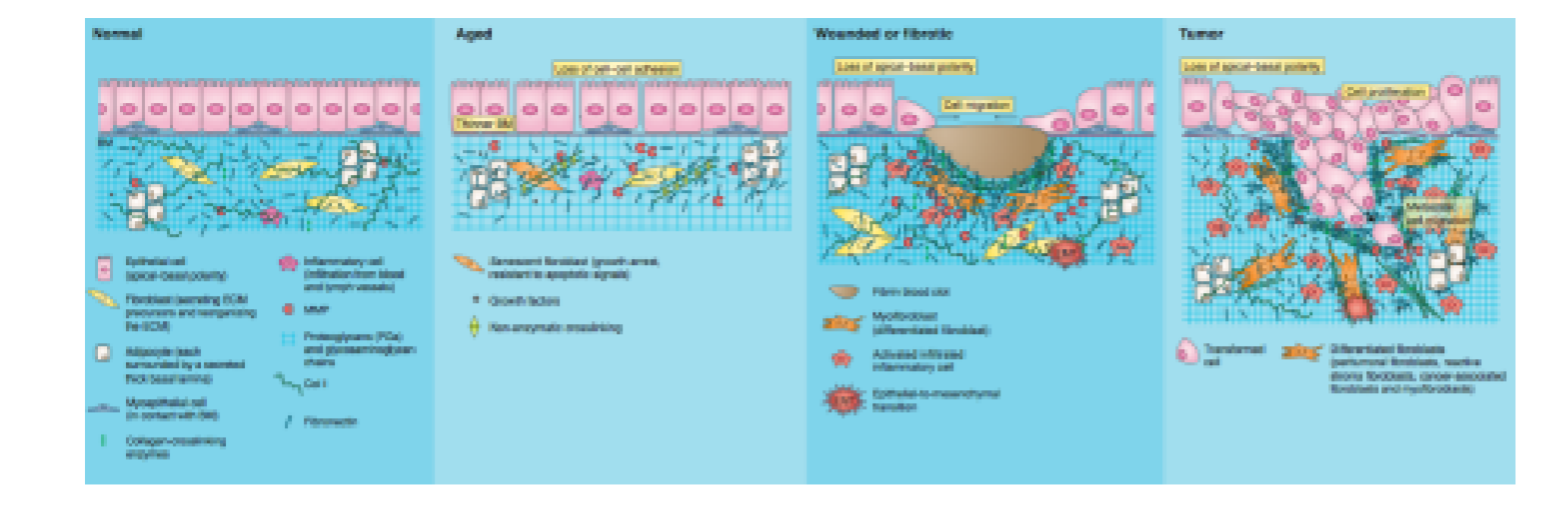
\includegraphics[width=1\textwidth]{ECMfunction.png}
\caption{\label{fig:ECM} ECM functionalization}
\end{figure}
Figure \ref{fig:ECM}:the first example is a normal situation, good substrate. In an aged person we have a loss of elasticity. In the case of a wound, we observe a coagulation cascade and scar tissue formation - which is characterized by a compact tissue. The temporary material (crust) is used as scaffold. We can have healing by repair or regeneration. There is a higher rigidity in the case of temporary material. In the case of a tumour, we have an abnormal growth and migration inside - which they should not be present. The migration is caused by fibers not organising to close the hole.

\subsection{Surface chemistry: biorecognition in ECM}
Cell biology is governed by a complex series of interactions with the ECM. It is not enough to promote proliferation, we should control the adhesion involving the integrins (connected with few genes). We need a pool of molecules, since biological functions are orchestrated by a symphony of signals. Communication between cells and the cellular matrix is very relevant.
\\
\\
\noindent
A \textbf{biomaterial} is a substance that has been engineered to take a form which, alone or as a part of a complex system, is used to direct, by control of interactions with components of living systems, the course of any therapeutic or diagnostic procedure in human or veterinary medicine.
The aim is to recreate a basic environment before inducing regeneration. We need to upregulate proliferation at the beginning to create a population, then stop it for reaching ECM formation and achieving a therapeutic impact. 
\noindent
Cells can interact moving molecules through the gap junctions or through integrins; there are cells that must be very close e.g. skin, myocardium, in other cases integrins are mandatory. The ECM should also provide security for travelling molecules,  as molecules should not be degraded and must be kept in the active conformation. 
Nutritional status is the bottle neck of tissue engineering, because in big wounds it is difficult to provide nutrition - as we need angiogenesis in order to have it. Hydrogels are cool because they can provide a lot of these requirements and can be combined to provide also mechanical support.
\\
\\
\noindent
The cell language is based on a mapping (micro- and nano-patterning) of biopolymers (dynamic ECM) shapes to their complementary binding. Chemical process during cell activity:
\begin{itemize}
\item Chemical reactions (irreversible): provide free energy (ATP $\rightarrow$ ADP)
\item Biopolymer (ECM) shape changes (reversible): provide control over chemical reactions
\end{itemize}

\subsection{Biocompatible materials: foundation ideas}
In order to design suitable materials, we should learn the biological pathways that lead to normal healing and reconstruction. Secondly, it is required to develop bio recognition surfaces that turn these pathways on and off. It is necessary to know specific affinities for the key molecules found in healing wounds that are associated with vascularised healing and regeneration (triggering local “unnatural” local healing).
If biomolecules are immobilised at the surface, they must be in the correct orientation and conformation. Porosity should be engineered to induce vascularisation and less fibrotic tissue. Furthermore, the modulus matching of scaffold-biomaterial should match with their intended use (modulus mismatch should exacerbate the FBRx).
Lastly, the engineered scaffold should be able to degrade into non-reactive substances at predetermined degradation rates to serve as a temporary guide for healing.

\section{Cell interactions}
Cells interact with the environment thanks to soluble factors, extracellular matrix and receptors.
Signals form ECM and neighbouring cells:
\begin{itemize}
\item gene expression regulation leads to adult stem cell differentiation [into the lineage of interest e.g. osteoblasts in bone]
\item tissue specific differentiation
\item survival of primary cells
\item Interaction with apoptosis: under external stimuli the cells may go to apoptosis. This may be useful in case of chemotherapy
\end{itemize}
The interaction between cells and matrix can be compared to a chemical reaction, where reagents can give rise to a reaction in a specific condition. Reactants are the cell + matrix, the specific condition is the biorecognition, we need integrins [without the plus (“+”) there is no reaction. All the reactants must communicate with each other. Integrins are important for response]. 
In order to achieve regeneration, we need to activate a number of functionalities, which should be listed according to time. The scaffold is a reactant, it is added in the bioreaction. Of course we also have mechanical stresses involved in the reaction. We need to take into account the control system, which should not be downregulated e.g. activate tissue regrowth and activate control system to stop when the tissue volume is enough. 

\begin{figure}[h]
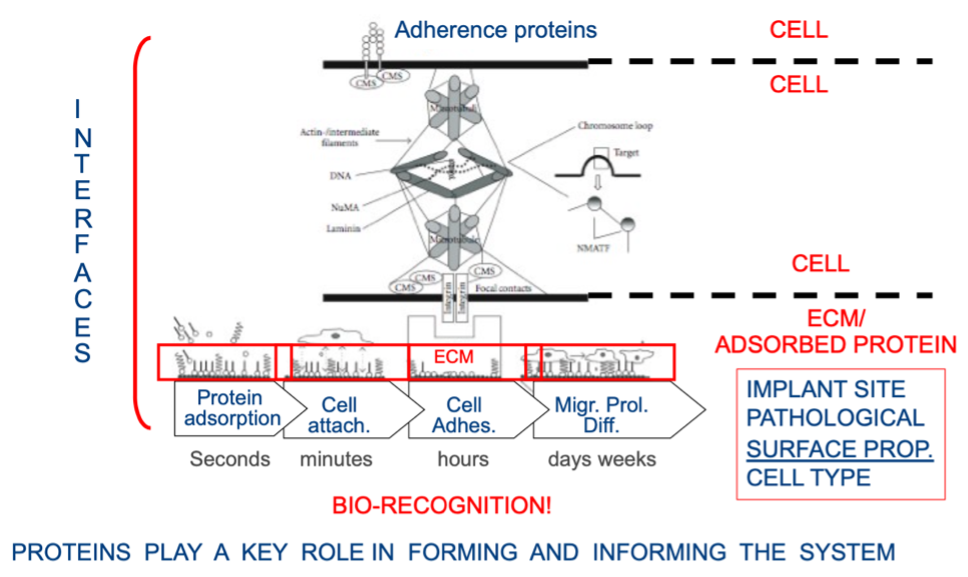
\includegraphics[width=1\textwidth]{interfaces}
\caption{\label{fig:interfaces}}
\end{figure}

\noindent
How does the body respond to the material?
Cells are in suspension in the culture, which contains serum (proteins). The surface first absorbs a coating of ions and proteins/lipids, which are then recognized and bound by cells.
Which kind of proteins will be absorbed by the implant? The quality of proteins depends on the chemical/mechanical properties of the scaffold and the context e.g. blood, skin, brain…For sure the first protein absorbed will be taken by plasma when we have bleeding. Depending on the proteins selected, the cells will adhere when the integrins of the cells can find some ligands among the proteins absorbed. 
We only have cell adhesion when we have biorecognition of the scaffold.
\\
\\
\noindent
Surfaces must be designed in order to control protein absorption. Depending on the phenotype, we have different groups of integrins and also integrins specific for different genes.
The aim of TE is to promote cell adhesion through specific integrins needed to achieve regeneration. Scaffolds and cells are not isolated,  the empty spaces are filled by the ECM (providing proteins and water). This first step is crucial, depending on this we will reach failure or success. Therefore, the surface of the scaffold is really relevant. We can change the chemical properties, functionalize with new chemical groups, modify morphology to drive the interaction between scaffold and cells.
The interaction between the implant and biological systems is a dynamic process. The biomaterial is characterized by specific properties. If we incubate the material in a single protein solution, where the protein is in active conformation. Depending on the surface properties, the biomaterial will absorb the proteins, which will remain active, or we will witness deactivation / degradation / modification. 
\begin{enumerate}
\item Protein is absorbed with original conformation = still active
\item Denaturation during absorption = not active, switch off
\item Different conformation = different activity [dangerous, unexpected situation]
\item Degradation = no specific activity, negative response and inflammation [small pro-inflammatory peptides are released into the environment]
\end{enumerate}
Having the protein active/inactive could be both positive or negative, it depends on what we need, what we want. The protein absorption mechanism is very dynamic, the absorbed proteins can also be released.
\\
\noindent
The protein substrate is important, we can change the material and see how it behaves.
We could observe different interactions with the proteins according to the starting material.Biocompatibility is a two-way process, the host affects the implant and vice versa. Also depending on the domain we will have a different adhesion, we can find differential adhesion distribution.
\\
\\
\noindent
\begin{figure}[h]
\centering 
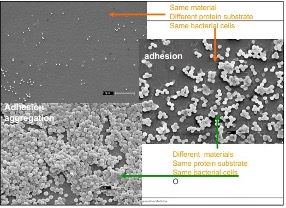
\includegraphics[width=0.5\textwidth]{polyu}
\caption{\label{fig:polyu}}
\end{figure}
Figure \ref{fig:polyu}: the aim was to produce a surface avoiding bacterial infection. The polymer is polyurethane, used for catheter production - antibacterial properties are really required. 
We see that the surface in contact with different protein substrates leads to different adhesion levels. When instead the protein substrate is equal with different materials, we see either adhesion or adhesion aggregation. 
\\
\\
\noindent
\begin{figure}[h]
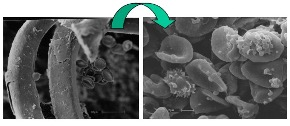
\includegraphics[width=0.5\textwidth]{vascular}
\centering
\caption{\label{fig:vascular}}
\end{figure}
Figure \ref{fig:vascular}: vascular graft that failed after 6 years of implantation. The implant failed because the surface was completely destroyed. The bacterial cells (there was infection) adhered to the implant and this activated inflammatory response. Inflammatory cells digested the implant, made of a really strong polymer (same as parachutes). In addition, the implant started to detach in the circulation system + bacteria were able to attach to red blood cells. This is one of the few cases in which we do not want cell adhesion.

\subsection{Molecular mechanism of cell adhesion}
The orientation of ligands is critical for cell adhesion and biological function. The RGD sequence promotes cell adhesion and it is usually included in a long peptide – to avoid that RGD is involved in the link between cells, it would be invisible. Depending on the protocol parameters, we can achieve a nice or absent adhesion. The density is the same, the only difference is the orientation.
For instance we could have a different density of signal,  leading to a different outcome in adhesion. The density of signal is important for the function.  Our aim is to reach an equilibrium, not too much or too little adhesion. In the second scenario the cell is able to move, good choice if cells are required to migrate into the scaffold. If instead we need a fast formation of a layer we can choose the first case.
No absorption = no adhesion at all. This may be useful in some cases, e.g. in blood vessels to prevent thrombus, release of proteins from nanoparticles in cancer treatment. 
Cell adhesion is mainly controlled by the surface. How can we know whether the conformation and orientation is correct? We can employ cell sensors, screening.

\begin{figure}[h]
\centering
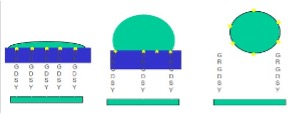
\includegraphics[width=0.5\textwidth]{adhesion}
\caption{\label{fig:adhesion}}
\end{figure}

\subsection{Cell adhesion}
Cell adhesion is a tightly regulated and dynamic biological process. It is central to physiological and pathological processes and critical to biomedical and biotechnological applications.
Adhesive interactions involve:
\begin{itemize}
\item anchorage (promotes migration, tissue organisation)
\item signaling (promotes activation, survival, proliferation, differentiation) 
\end{itemize}

\begin{figure}[h]
\centering
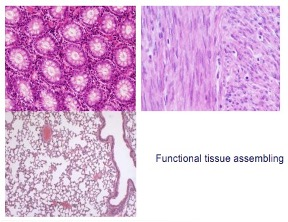
\includegraphics[width=0.5\textwidth]{functionaltissue}
\caption{\label{fig:funtis}}
\end{figure}

In figure \ref{fig:funtis} starting from top left we see the functional tissue assembling of glands (radial section), muscles, and lung/alveolar tissue. In the case of muscles, functional tissue should support mechanical stress. In glands we have cells forming very well polarized tubes for transport, which are called capillary tubes. For lung tissue we have blood vessels, we need to have a small surface and permeability for gas exchange. The air should move into the bloodstream,  so the tissue should be very thin and adherent to the vessels. We have a low amount of ECM, the mechanical support is provided by cells themselves. The structure is function-dependent. 
Assembly is driven by ECM and adhesion patterning. The morphology should depend on the function. Thin layer of ECM in the basal lamina, collagen fibrils. This provides elasticity, the fibrils are not a bundle, but organise somehow.


\subsection{Cell-material interactions}
Cells cannot adhere to synthetic surfaces, as there is no biorecognition (ECM performs better).
Cell adhesion to synthetic and bio surfaces occurs through a specific receptor interaction with adhesion protein/motifs:
\begin{itemize}
\item proteins adsorbed from physiological fluids (fibronectin, vitronectin, fibrogen)
\item ECM components present or deposited by cells (fibronectin, collagen, laminin)
\item biospecific sequences engineered on surfaces (RGC,YIGSR) for biorecognition
\end{itemize}
Adhesion receptor families are cadherins, selecting, HSPG, integrins, Ig superfamily.
Specific integrins act on specific receptors, so we must be precise. For instance, alpha5beta3 can recognize the ligands into fibronectin, collagen is recognize by alpha2beta1. 
\noindent
FIG
How to measure the adhesion strength of the cells? Experiment by Gallant and Garcia (2003). They provided two samples, performed centrifugation and measured cells attached and cells not adhered. In this way you can measure the difference in the strength of the adhesion.
\\
\\
\noindent
Depending on the surface chemistry, we will have a different cell adhesion rate.  According to the protein coating, e.g. either fibronectin or type I collagen, we will have different biological performance. A number of evaluation methods can give us an idea of the adherence strength.
\\
\\
\noindent
Figure \ref{fig:fibrin} design scaffold for neuron regeneration. Adhesion is necessary, but neurons also need to form connections with other neurons. RGD goal: neurite outgrowth, strategy: RGD- functionalization. They provided the material with fibrin, fibrin with low RGD and fibrin with high RGD. RGD is the classical adhesion peptide. 
\begin{figure}[h]
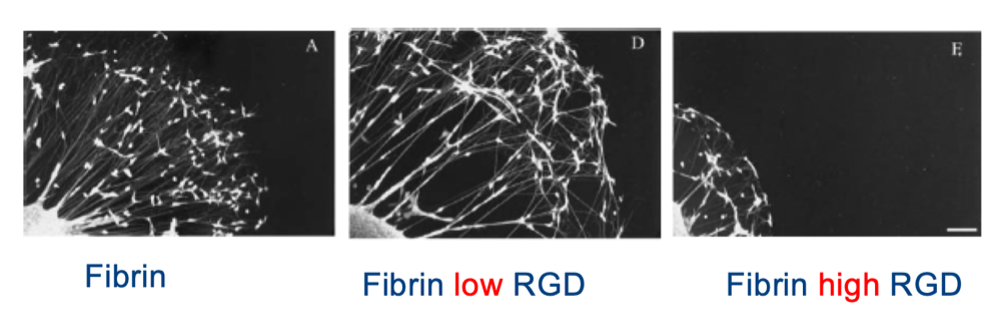
\includegraphics[width=1\textwidth]{fibrin}
\caption{\label{fig:fibrin}}
\end{figure}
\noindent
We observe a different response: high density is too much,  instead with a low amount of RGD we have a good outcome with a huge number of connections. When we increase RGD, the surface becomes more adhesive; this is mainly due to the fact that the cells are too sticky, but also because we must reproduce a biological environment. The amount of RGD should resemble the natural one. In fibronectin, the RGD content is 1 per chain, low amount. We have to move inside the natural range of pH, etc, … We want natural conditions. The language of the cells cannot be changed, we have to adapt our language. Signal is the combination of the ligand and density.
 \\
 \\
 \noindent
Adhesion is completely different in 2D and 3D. Cell adhesion is characterized by three stages: attachment cell body, flattening and spreading, and organization of the actin skeleton with the formation of focal adhesion between cell and its substrate. The strength of adhesion becomes stronger with the length of time a cell is allowed to adhere to a substrate or another cell. 

\subsection{Cell organization}
The cell's adhesive interactions with the surrounding ECM (number of adhesive motifs, distribution, density) and neighbouring cells define cell shape and organisation, controlling functionality. This environment regulates the cell survival, differentiation, proliferation and migration.
\\
\\
\noindent
Chondrocytes are exposed to compressive forces, interstitial fluid flow and adhesive cues (cytokines) for cartilage maintenance. Chondrocytes are in a lacuna, they should behave like pillars and maintain their shape.
Soluble and matrix-bound GFs and flow induced mechanical forces on blood vessel wall, endos after polarity, cell-cell contacts, and degrade the surrounding basement membrane and stromal ECM in order to migrate and form tubular sprouts. 
Adhesive and mechanical cues drive cell organization. Misregulation of the mechanism induces mechanical and structural changes in the ECM, and transformed epithelial cells migrate towards vasculature and eventually metastasize.
\\
\\
\noindent
ECM-dependent regulators can be associated with 2D, 1D and 3D migration. In turns influence intracellular pathways that govern the migratory phenotype. 3D are characterized by pore size and interconnection (cross linking degree). Aligned fibers are randomly distributed with low density in the scaffold.
\\
\\
\noindent
Adhesion and migration are controlled by the ECM composition, stiffness of the material and ligand density. While using fibers, something changes: by having a new parameter, aligned topography, we obtain different architectures. In the case of a mixed fibrous scaffold, we also have aligned/random, elastic behaviour, cross linking. Sending seed cells on the different structure, we will se diverse behaviour for orientation, migration, etc. Architecture can play a huge role.
\\
\\
\noindent
The substrate contractility regulates 3D migration, regardless of pore size. Stiff fibers vs soft fibers: when the cell lands on stiff fiber it can adhere, but becomes very stable and not able to modify the body/migrate. Instead cells on soft fibers are able to move and form protrusions.
Since cells in nature are connected to ECM fibers, when they move the ECM will also follow the contraction of the cell body. If the cell adheres to the soft fiber, the same natural movement can occur. When the substrate is too rigid contraction cannot occur, healing will be different. The scaffold should be soft enough to follow the reorganization needed by the cells.
\\
\\
\noindent
\begin{figure}[h]
\centering
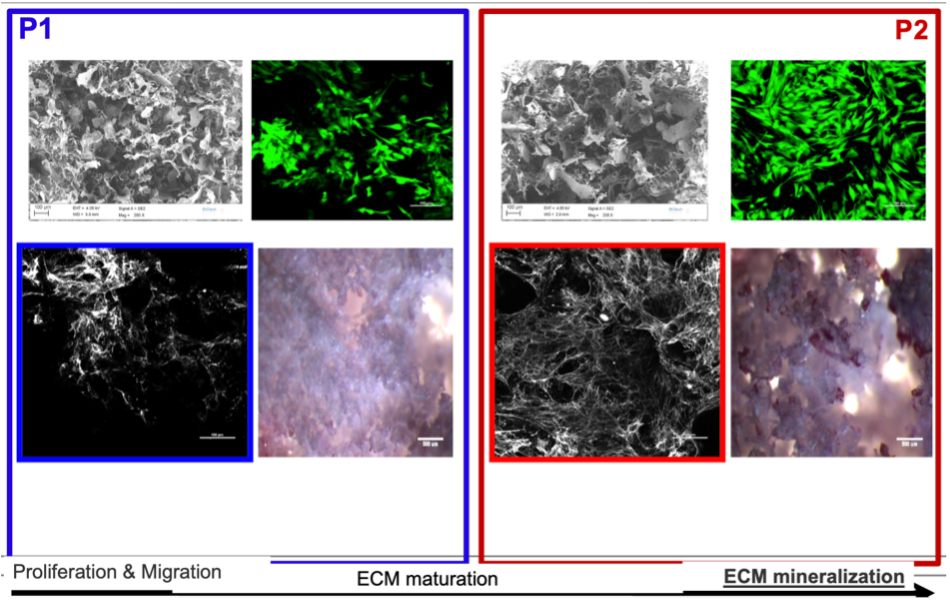
\includegraphics[width=0.7\textwidth]{mineralization}
\caption{\label{fig:min}}
\end{figure}
Figure \ref{fig:min}: two scaffolds prepared with the same polymer, the difference is in pore size and distribution. The scaffolds are built for bone regeneration; we should take into account the presence of collagen fiber in a continuous network. Osteoblasts should infiltrate the scaffold for building the network, porosity should allow this. Once the network is formed, we have the deposition of the hydroxy apatite on top of collagen fibers.
Difference between P1 and P2 in terms of cell distribution: in P2 uniform, in P1 clusters (interconnection not complete). When we observe clusters of cells, we expect that the osteoblasts are not able to build a continuous network, due to tight collagen + no mineralization. When cells are not able to migrate, mineralization cannot occur. 
A continuous network is also required for capillary formation. The parameters can be fully controlled with scaffold design. In order to improve the performance of P2 scaffold we could functionalize it with collagen or drug release systems.
\\
\\
\noindent
The scaffold surface interacts with the cell through the ECM (biorecognition). Our aim is to reproduce in vitro a working environment, working for the cell and solving a specific task. Depending on the context, we can have the bioreaction: the cell recognizes the surface of the scaffold if it is functionalized or for protein absorption. We have to refer to the cell population we are interested in, we have specific integrins. 

\subsection{Methods for modulating receptor-ligand interactions}
\begin{enumerate}
\item Natural ECM biomaterials: biologically relevant environment, but poor mechanical properties and inconsistent reproducibility
\item Whole ECM adsorption
\item Synthetic linear binding motif: surface functionalization. We need to define the density of the signal, the protein of interest , the stability (quantify the time for which the signal should remain, orientation, homogeneous or pattern distribution.
\item Spatially oriented binding motif
\item Nanopatterning with nanolithography: mix different molecules and patterns, as well as technologies
\item ECM-like biomaterials
\end{enumerate}


\end{document}



  % Add appendix if needed

\end{document}
